
% 
% Annual Cognitive Science Conference
% Sample LaTeX Paper -- Proceedings Format
% 

% Original : Ashwin Ram (ashwin@cc.gatech.edu)       04/01/1994
% Modified : Johanna Moore (jmoore@cs.pitt.edu)      03/17/1995
% Modified : David Noelle (noelle@ucsd.edu)          03/15/1996
% Modified : Pat Langley (langley@cs.stanford.edu)   01/26/1997
% Latex2e corrections by Ramin Charles Nakisa        01/28/1997 
% Modified : Tina Eliassi-Rad (eliassi@cs.wisc.edu)  01/31/1998
% Modified : Trisha Yannuzzi (trisha@ircs.upenn.edu) 12/28/1999 (in process)
% Modified : Mary Ellen Foster (M.E.Foster@ed.ac.uk) 12/11/2000
% Modified : Ken Forbus                              01/23/2004
% Modified : Eli M. Silk (esilk@pitt.edu)            05/24/2005
% Modified : Niels Taatgen (taatgen@cmu.edu)         10/24/2006
% Modified : David Noelle (dnoelle@ucmerced.edu)     11/19/2014

%% Change "letterpaper" in the following line to "a4paper" if you must.

\documentclass[10pt,letterpaper]{article}

\usepackage{cogsci}
\usepackage{pslatex}
\usepackage{apacite}
\usepackage{amsmath,amssymb}
\usepackage{graphicx}
\usepackage{color}
\usepackage{url}
%\newcommand{\url}[1]{$#1$}


\definecolor{Red}{RGB}{255,0,0}
\newcommand{\red}[1]{\textcolor{Red}{#1}}

 \newcommand{\denote}[1]{\mbox{ $[\![ #1 ]\!]$}}


\newcommand{\subsubsubsection}[1]{{\em #1}}
\newcommand{\eref}[1]{(\ref{#1})}
\newcommand{\tableref}[1]{Table \ref{#1}}
\newcommand{\figref}[1]{Figure \ref{#1}}
\newcommand{\appref}[1]{Appendix \ref{#1}}
\newcommand{\sectionref}[1]{Section \ref{#1}}

\title{Animal, dog, or dalmatian? Contextual informativeness, utterance length and utterance frequency affect choice of referring expressions.}
%\title{Wonky worlds: Listeners reconsider world knowledge when utterances are odd}
%Non-sinking marbles are wonky: defeasible world knowledge in language interpretation}

 
\author{{\large \bf Caroline Graf, Judith Degen, Robert Hawkins, Noah D.~Goodman} \\
  cgraf@uos.de, \{jdegen,rxdh,ngoodman\}@stanford.edu\\
  Department of Psychology, 450 Serra Mall \\
  Stanford, CA 94305 USA}



\begin{document}

\maketitle


\begin{abstract}

\red{The choice of referring expressions is highly context dependent. Whether speakers choose to refer to an object as a “dalmatian", a “dog", or an “animal" is determined partly by the features of the other objects present in the scene, as well as features of the utterance alternatives. The current study within a reference game setting demonstrates that speakers' choice of referring expression is dependent on a rich interplay of the expression's degree of contextual informativeness, its relative length and its relative frequency. If a competitor object of the same category (e.g., dog) as the target object is present in the display, speakers choose a more specific subcategory (e.g., “dalmatian") to refer to the target object. In contrast, when the competitor objects do not share the same (super-) category as the target, speakers are less constrained in choosing an appropriate referring expression. In this event, shorter expressions are preferred over longer ones and more frequent category names are preferred over less frequent ones. The pattern of results is predicted by a production model couched in the Rational Speech Act framework, in which a speaker is modeled as balancing an utterance's contextual informativeness with its cost relative to its alternatives.}

\textbf{Keywords:} 
referential expressions, levels of reference, overinformativeness, basic levels, categorization
\end{abstract}

\section{\bf Introduction}
One of the main purposes of language is communication. In fact, some cognitive scientists have gone as far as proposing that language may simply be a special case of social cognition: Speakers choose an utterance approximately optimally such that a listener can infer the intended meaning by means of Bayesian inference (Goodman and Stuhlmueller, 2012). According to this view, language is essentially about reasoning about other people's knowledge, states and intentions. An important assumption here is that the speaker is a rational agent, who selects an utterance based on its optimal expected utility. 

Although approaches in this framework have been increasingly successful in predicting human behavior, past research in the area of referential expressions has demonstrated that speakers are not necessarily behaving in a rational manner when it comes to producing referential expressions. For instance when subjects tend to overly produce color modifiers to describe objects, even if color is not an attribute necessary for disambiguation (e.g. Pechmann, 1989; Sedivy, 2003). For example, when subjects are being shown a small red cup as a target object in the context of a big red cup and a big blue cup and asked to describe the target, a significant amount of subjects say “small red cup", when “small cup" would have been sufficient for disambiguation. Speakers are producing overinformative utterances and can thus be said to be irrational in their behavior (Gatt et al., 2012). 

Furthermore, in terms of levels of reference it has been established that speakers have a strong preference for the basic level of reference when describing objects (Rosch, 1976). That is, when asked whether to call an object a “dalmatian", a “dog" or an “animal" out of context, speakers favor “dog" over the other two alternative levels of reference. Seen in the light of overinformativeness, one might argue that speakers act in an overinformative manner when describing an object in a more specific way than is necessary for disambiguation, for example when saying “dog" in the above scenario instead of calling the object an “animal". But under what circumstances do speakers actually use the basic level and when do they revert to the sub- or superlevel? Which other factors contribute to the choice of utterance and is there a way to manipulate the speaker's behavior? 

Including more attributes than are necessary to identify a target object may at first seem to contradict the Maxim of Quantity by Grice (1975), namely to make one's contribution as informative than is required and not more, but what does it actually mean for an utterance to be more informative than *required*? Does it mean that this utterance mentions attributes redundantly irrespective of their utility? What if the so called “redundant" attributes (e.g. Arts, 2004; Arts, Maes, Jansen, & Noordman, 2011) actually have an utility after all by influencing the processing of an utterance? Pechmann (1985) has argued that the excessive use of color adjectives in referential expressions does in fact contribute to the informativeness of the utterance, namely by excluding some (but not all) distractors. As a matter of fact, other studies have demonstrated that overspecified utterances give rise to shorter identification times compared to minimally specified expressions (Deutsch, 1976; Sonnenschein, 1982). Thus, “overinformative" behavior must not necessarily be irrational behavior. 

A similar argument can be made for the the use of a level of reference less abstract than necessary for disambiguation and the dominance for the the basic level in the production of referential expressions. The basic level of reference, which Rosch et. al (1976) characterize as the level of abstraction at which the most basic category cuts are made, seems to have a special status in human categorization behavior: Basic level categoriy labels are not only the first labels used for categorization during perception of the environment, but also the labels which lead to fastest category verification. Basic levels also carry the most information and possess the highest category cue validity (compared with the sublevel “dalmatian" or superlevel “animal"). Therefore it can be argued that being more specific than necessary has a positive effect on the processing of the utterance for the listener and thus “overinformativeness" contributes to the informativeness of the utterance.

The following experiment explores what effect context has on the choice of referring expression by varying the level of reference of the distractor objects; distractors may be from the same basic level category or the same super level category as the target object or belong to neither. Furthermore we investigate whether and under what circumstances the basic level is preferred, how important of a role informativeness plays and what specific aspects of the labels, particularly length and frequency, are other factors contributing to the selection of utterance. 

\section{\bf Methods}

\subsection{\bf Participants}
We recruited 56 participants over Amazon’s Mechanical Turk, who were all native speakers of English and who were reimbursed for their participation in the experiment. The subjects participated in pairs of two.

\subsection{\bf Materials}
Stimuli were selected from eight distinct domains. These domains represented basic level categories such as “dog”, for each of which four targets were chosen, which were subcategories of this domain (e.g. “dalmatian”, “pug”, “German Shepherd” and “husky”). Each domain also contained an additional item which belonged to the same basic level category as the targets (e.g. “greyhound”) as well as items which did not belong to the same basic level category, but to the same supercategory (e.g. “elephant” or “squirrel”). 

\subsection{\bf Design}
Each trial consisted of a display of three pictures of objects, one of which was designated as the target object. There were four target objects for each of the eight domains, each of which would appear once for every pair, giving rise to a total of 36 trials per pair. There were four conditions which differed in the types of distractors which were shown: (a) {\bf distractor12}: one distractor of the same basic level and one distractor of the same superlevel were present (e.g. target: “dalmatian”, distractor 1: “greyhound”, distractor 2: “squirrel”), (b) {\bf distractor22}: two distractors of the same superlevel were present, (c) {\bf distractor23}: one distractor of the same superlevel and one artifact were present and (d) {\bf distractor33}: two artifacts were present. The selection of distractors was random for each trial. Furthermore, the experiment contained 36 filler items, in which participants were also asked to produce referential expressions for objects, but here the three pictures illustrated the same stimulus which differed only in size and color. No filler items were reused in the target trials.

\subsection{\bf Procedure}
The experiment was conducted online within a reference game setting. Subjects participated in pairs and were either assigned the speaker or the listener role. Participants would keep their allotted roles for the entire experiment. They were informed that the order of the three pictures which they would both see will be different for the speaker and the listener. Only the speaker could identify the target object by a green square surrounding it. There was a chatbox in which speaker and listener could send messages to each other and communicate. The task was for the speaker to tell the listener which one of the objects is the target and for the listener in turn to select the right object based on this information provided by the speaker. 

\subsection{\bf Annotation}
Responses were parsed automatically and subsequently checked manually to determine the level of reference used. Incorrect trials were excluded from the analysis, which led to the elimination of 1,1\% of trials. Moreover, one analysis was done which included only the literal mentioning of the sub-, basic- and superclass, whereas another analysis also included responses naming the main attribute of a class (e.g. “can fly” for “bird” was counted as mentioning the basic level category). 

\section{\bf Results}

\subsection{}
As shown in Fig. 1, speakers are most  likely to refer to the target object with a subcategory label, if their choice of utterance is constrained by a distractor of the same basic level category as the target being present in the scene (i.e. condition distr12, e.g. target: “dalmatian”, distractor 1: “greyhound”). However, when there is no other object of the same basic level category present (as in conditions distr22, distr23 and distr33), subjects are far more likely to choose the basic level term. Interestingly, use of the subcategory term decreases further as there are less or no other distractors present which belong to the same supercategory (e.g. animal). That is, participants are less likely to say “Dalmatian” when there is another animal and an artifact in the display opposed to when there are two animals in the display, and even less likely to say “Dalmatian” when there are no animals in the display. Similarly, the use of the basic level expression steadily increases as the number distractors of the same supercategory decreases. Naming the object by its supercategory term is far less probable than using either the sub- or basiclevel terms, but also increases as the constraints on the speakers utterance choice decrease. Statistical analyses confirmed a main effect of condition...

\begin{figure}[ht!]
\centering
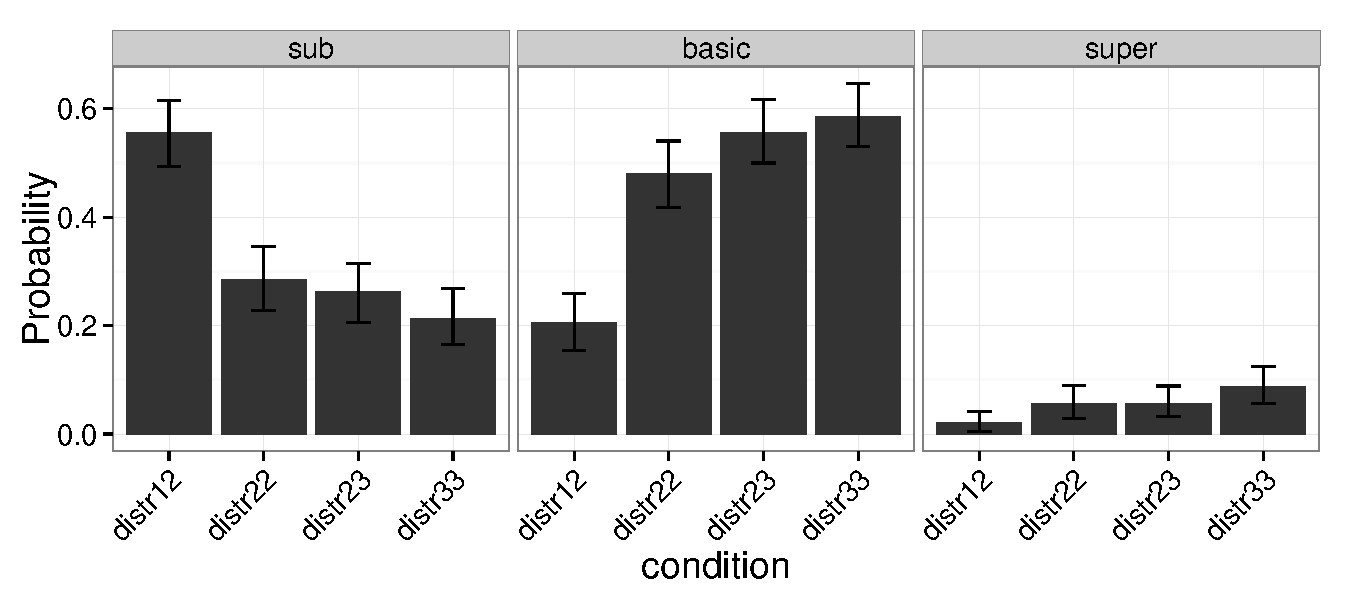
\includegraphics[width=90mm]{graphs/proportion_mentioned_features.pdf}
\caption{Figure 1: Histogram of probabilities of mentioning the sub-, basic- or superlevel category \label{overflow}}
\end{figure}

\subsection{\bf Domain-specific results}
The overall effects were slightly different in the different domains (see Fig. 2). For instance, mentioning the subclass over the basic level term was preferred more in some domains (e.g. in the “candy” domain) than in others. Likewise, some domains had a greater preference for basic level terms (e.g. the “shirt” domain). Using the superclass term also ranged from hardly being observable (e.g. the “flower” domain) to being used more frequently (e.g. in the “bird” domain). Nevertheless, mentioning the sublevel category was always the most frequent choice of utterance in the case where a distractor of the same basic level was displayed. Furthermore, the sublevel term was always mentioned most frequently and the basic level least frequently in just this condition, compared to the other three conditions.

\begin{figure}[ht!]
\centering
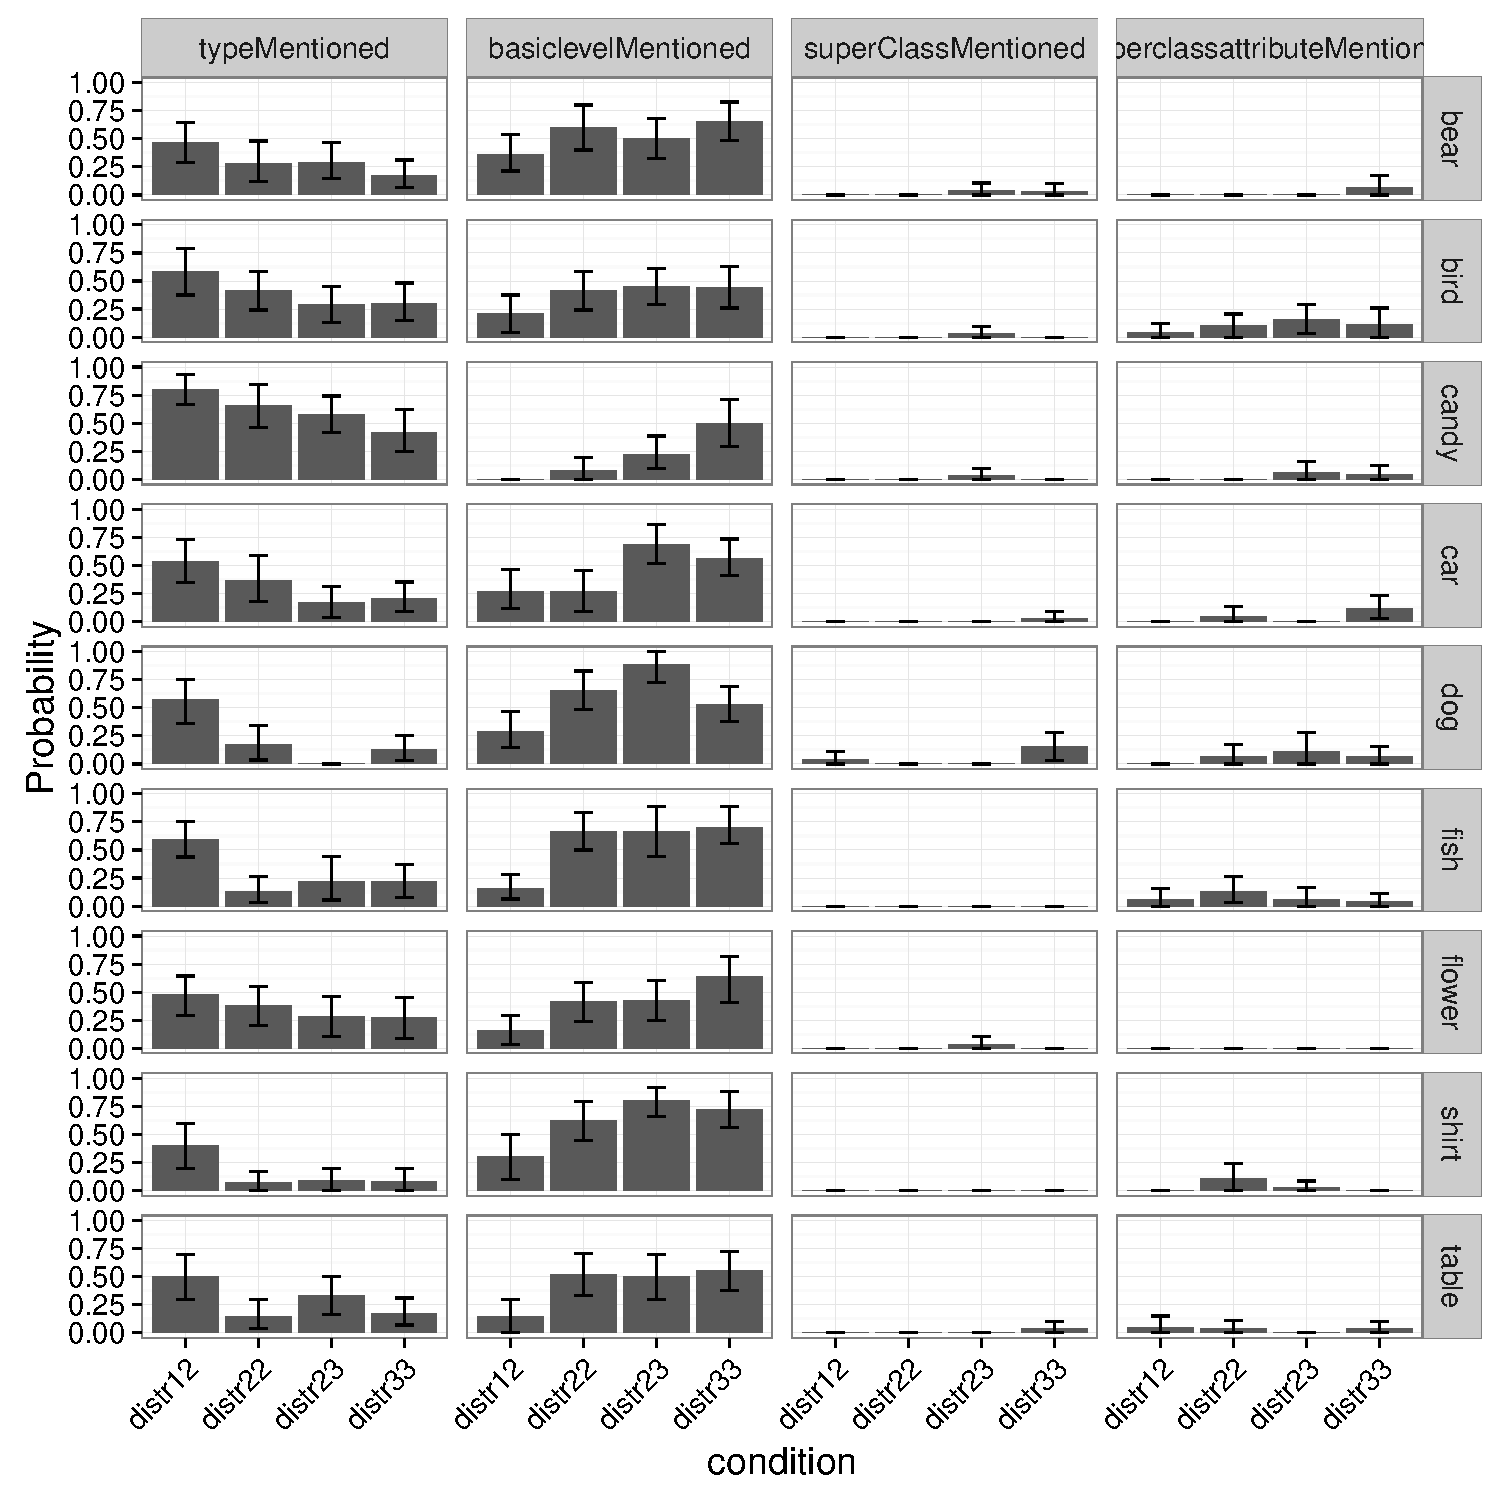
\includegraphics[width=90mm]{graphs/proportion_mentioned_features_by_domain.pdf}
\caption{Figure 2: Domain-specific histogram of probabilities of referring to targets with sub-, basic- or superlevel term \label{overflow}}
\end{figure}

\subsection{\bf Utterance length}
Another factor contributing to the selection of a level of reference is relative utterance length. As displayed in Fig. 3, speakers are more likely to use the subcategory term if it is relatively short compared to the basic level term (i.e. the ratio sub/basic is relatively small, see blue bars in sublevel column). For example, the length ratio of “chihuahua”/”dog” is bigger than that of “pug”/”dog”, thus the data suggests that “chihuahua” is less frequently used than “pug”. This effect was independent of whether the use of the subcategory was forced by a distractor of the same basic level in the context or not. Furthermore, if the subcategory term was relatively long compared to the basiclevel (i.e. the sub/basic ratio is relatively big, see red bars in basic level column), subjects are more likely to use the basic level referential expression. Statistical tests confirmed

\begin{figure}[ht!]
\centering
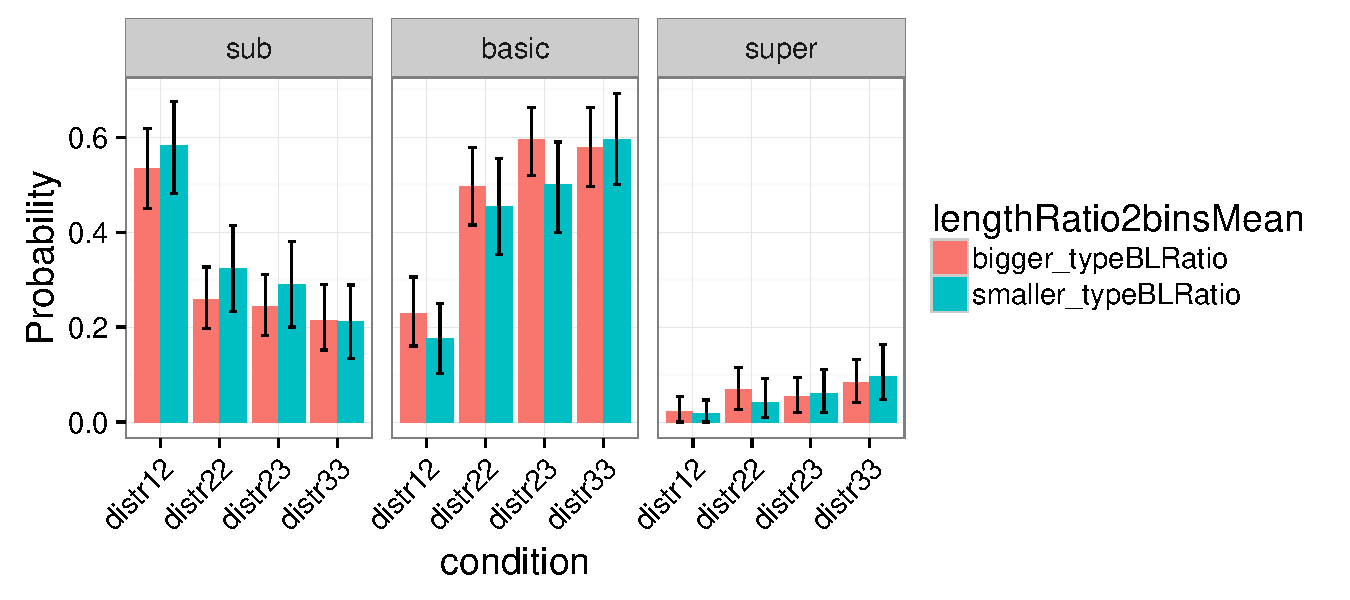
\includegraphics[width=90mm]{graphs/lengthRatio.pdf}
\caption{Figure 3: Probability of using sub-, basic- and superlevel terms when the sublevel/basiclevel length ratio is bigger (red) or smaller (blue) than the mean  sublevel/basiclevel length ratio \label{overflow}}
\end{figure}

\subsection{\bf Utterance frequency}
Besides contextual informativeness and utterance length, the frequency of a specific label also plays a role in determining speakers choice in referential expression. Illustrated in Fig. 4, the data suggests that relatively frequent sublevel terms (i.e. those which have a relatively high frequency compared to the frequency of the basic level and thus also have a relatively big frequency ratio) are preferred over more infrequent ones. This is especially the case when the speaker is not forced to use the subcategory term, namely when there is no distractor present which is a member of the same basic level category as the target (conditions distr22, distr23 and distr33). The basic level terms on the other hand are used more often if the competing sublevel alternative is relatively infrequent (see blue bars in basic level column). ...

\begin{figure}[ht!]
\centering
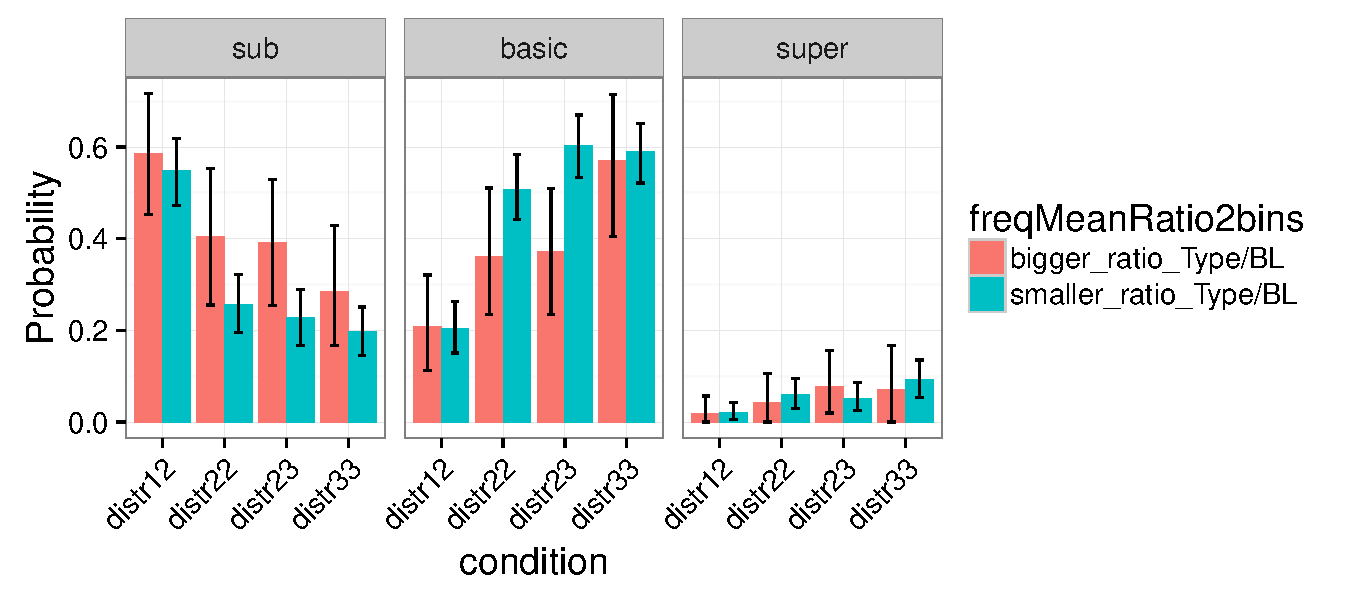
\includegraphics[width=90mm]{graphs/frequencyRatio.pdf}
\caption{Figure 4: Probability of using sub-, basic- and superlevel terms when the sublevel/basiclevel frequency ratio is bigger (red) or smaller (blue) than the mean  sublevel/basiclevel frequency ratio \label{overflow}}
\end{figure}

\subsection{\bf Interaction between length and frequency}
Furthermore, there was an interaction between length and frequency, such that length had a greater effect on high-frequency than on low-frequency sublevel terms...

\begin{figure}[ht!]
\centering
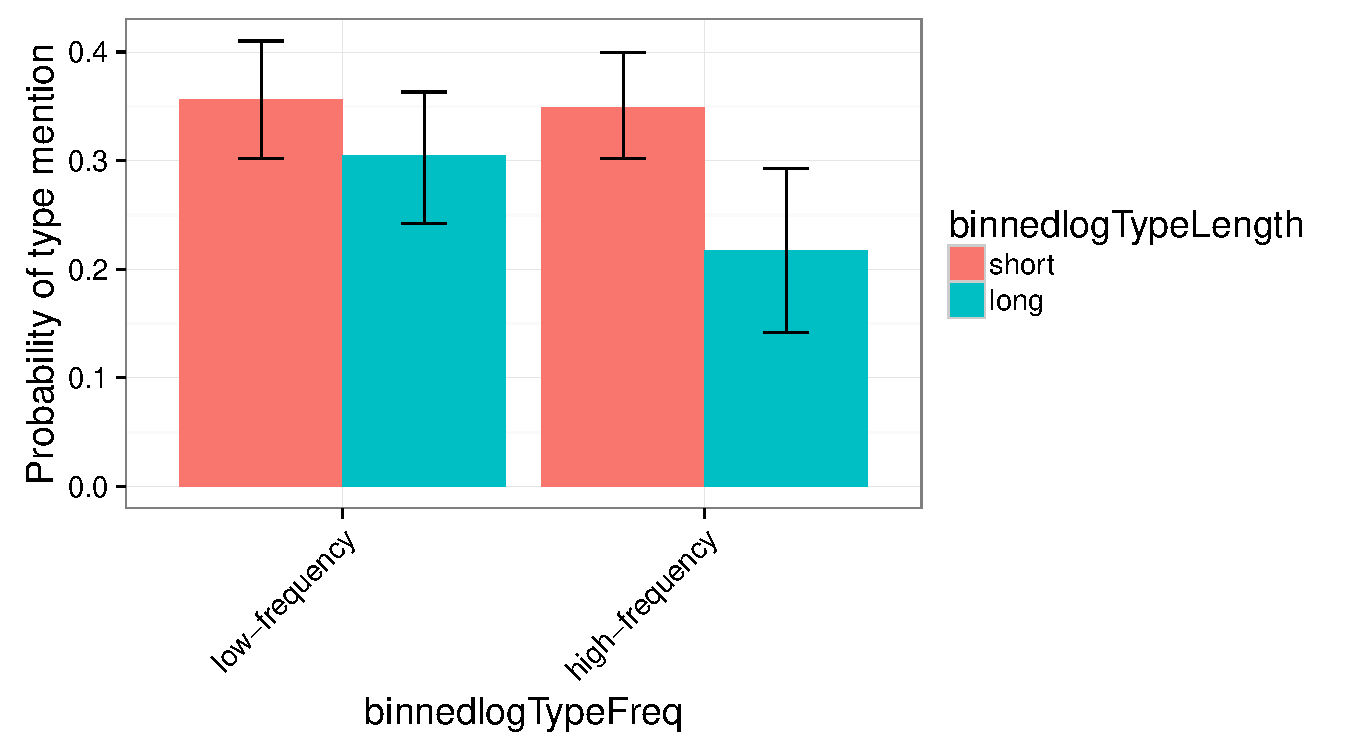
\includegraphics[width=90mm]{graphs/freq-length-interaction-noconds.pdf}
\caption{Figure 5: Probability of using a sublevel term when its frequency is high opposed to low and the length short opposed to long, averaged over conditions \label{overflow}}
\end{figure}

\section{\bf Modelling the choice of referential expression in RSA}

\section{\bf Discussion and conclusion}

\section{\bf Acknowledgments}

This work was supported by ONR grant N00014-13-1-0788 and a James S. McDonnell Foundation Scholar Award to NDG and an SNF Early Postdoc.Mobility Award to JD.

\small


\bibliographystyle{apacite}

\setlength{\bibleftmargin}{.125in}
\setlength{\bibindent}{-\bibleftmargin}

\bibliography{bibs}


\end{document}
